% !TEX root = ../Thesis.tex
\myChapter{The mammalian lung}\label{ch:lung}
\begin{flushright}{\slshape I'm throwing rocks tonight. Mark it, Dude.} \\ \medskip
    --- \defcitealias{TheBigLebowski}{Steve Buscemi as Donny}\citetalias{TheBigLebowski} \citep{TheBigLebowski}
\end{flushright}
\bigskip
\section{Interestingness}
Why is the mammalian lung so interesting?

\section{Lung Development}
During lung development all the internal structures like the conducting airways, the blood vessel network and the gas exchange area are formed. The lung is specifically designed to provide this large gas exchange surface---in humans the alveolar gas exchange surface is in the order of \SI{130}{\meter\squared}, an area equivalent to about $\frac{3}{4}$ of a tennis court~\cite{Weibel2009}---where capillary blood efficiently gets in close contact to the air inside the lung structure. 

Mammalian lung development can be divided into five overlapping stages~\cite{Schittny2004,Schittny2007a}, as shown in figure~\ref{fig:lung development stages}: Organogenesis starts with a outpouching of the foregut resulting in the appearance of the lung buds and formation of the major airways. Subsequently, the conducting and parts of the respiratory airways are formed by a successive cycle of branching and growth starting at the lung buds, which is called branching morphogenesis. Most of this process takes place during the pseudoglandular stage. In this stage the functional respiratory lung unit, the so-called acinus is ``born''. An acinus is defined as the complex of alveolated airways distal of a last purely conducting airway, the terminal bronchiole~\cite{Rodriguez1987}. The total of all acini forms the lung parenchyma, the area where the pulmonary gas-exchange takes place.

\begin{figure}[htb]
	\centering
	\pgfplotsset{width=\linewidth,height=.5\linewidth}
	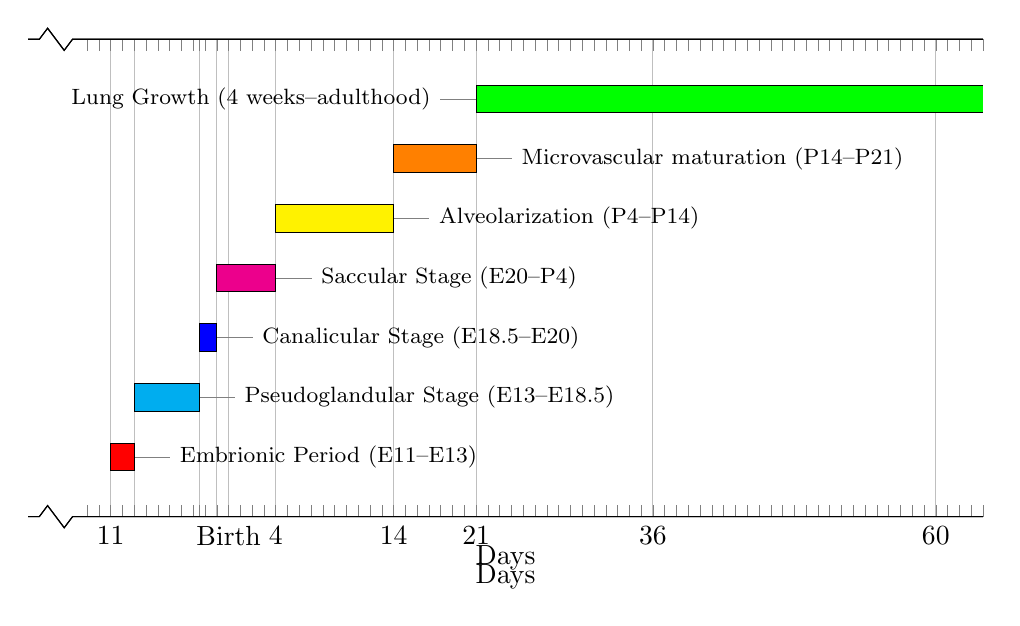
\begin{tikzpicture}
		\def\xmin{4}
		\def\xmax{85}
		\def\ymin{0}
		\def\ymax{0.4}
		\begin{axis}[xbar stacked,%
			scale only axis,%
			xmin=\xmin,%
			xmax=\xmax,%
			ymin=\ymin,%
			ymax=\ymax,%
			yticklabels={},%
			axis x discontinuity=crunch,%
			xtick={9,...,\xmax},%
			xticklabels={},
			xlabel=Days,%
			axis y line=none]
		\end{axis}
		\begin{axis}[xbar stacked,%
			scale only axis,%
			xmin=\xmin,%
			xmax=\xmax,%
			ymin=\ymin,%
			ymax=\ymax,%
			yticklabels={},%
			axis x discontinuity=crunch,%
			xtick={11,13,18.5,20,21,25,35,42,57,81},%
			xticklabels={11,,,,Birth,4,14,21,36,60},
			xmajorgrids,%
			xlabel=Days,%
			%axis x line=bottom,%
			axis y line=none]
			\def\step{0.05}
			\addplot [transparent]	coordinates {(11,0)};
			\addplot [fill=red]		coordinates {(2,1*\step)};
			\addplot [fill=cyan]		coordinates {(5.5,2*\step)};
			\addplot [fill=blue]		coordinates {(1.5,3*\step)};
			\addplot [fill=magenta]	coordinates {(5,4*\step)};
			\addplot [fill=yellow]	coordinates {(10,5*\step)};
			\addplot [fill=orange]	coordinates {(7,6*\step)};
%			\addplot [fill=green]		coordinates {(39,7*\step)};
			\addplot [fill=green]		coordinates {(\xmax-41,7*\step)};

			\tikzstyle{every pin}=[%
				%fill=white,%
				%semitransparent,%
				%draw=black,%
				%text width=10em,%
				font=\footnotesize,
				%text centered,%
				pin distance=3ex]
			\node[coordinate, pin=right:{Embrionic Period (E11--E13)}] at (axis cs:13,0.05) {};
			\node[coordinate, pin=right:{Pseudoglandular Stage (E13--E18.5)}] at (axis cs:18.5,0.1) {};
			\node[coordinate, pin=right:{Canalicular Stage (E18.5--E20)}] at (axis cs:20,0.15) {};
			\node[coordinate, pin=right:{Saccular Stage (E20--P4)}] at (axis cs:25,0.2) {};
			\node[coordinate, pin=right:{Alveolarization (P4--P14)}] at (axis cs:35,0.25) {};
			\node[coordinate, pin=right:{Microvascular maturation (P14--P21)}] at (axis cs:42,0.3) {};
			\node[coordinate, pin=left:{Lung Growth (4 weeks--adulthood)}] at (axis cs:42,0.35) {};
		\end{axis}
	\end{tikzpicture}
	\caption[Lung development stages]{Lung development stages for the rat lung. The first three stages (Embrionic Period, Pseudoglandular and Canalicular Stage) take place in the approximately 21 days from the beginning of gestation to birth. E=embryonic day (days post-coitum), D=postnatal day. Figure adapted from~\cite{Schittny2007a}.}
	\label{fig:lung development stages}
	\todo[inline]{Reference correct? I've nicked it from p:/\#Talks/2009.07.02 2ndYearExamination/Imaging-Goe-090515.ppt}
\end{figure}

The pseudoglandular stage is followed by intermediate stages, which are called canalicular and saccular. During the canalicular stage a first functional gas exchange surface---the air-blood barrier---is formed and the lung epithelium starts to differentiate. The saccular stage marks the switch from branching to septation morphogenesis.

During the alveolar stage the distal part of the bronchial tree is enlarged by the introduction of new alveoli through a formation of additional septa from already existing septa. 

In order to optimize gas exchange after bulk alveolarization is completed, the interalveolar septa and their capillary networks are remodeled during the phase of microvascular maturation. At this point lung development is considered as being finished and normal growth of the organ follows\graffito{The time point of birth differs between mammals, relative to the state of lung development. In humans, birth happens at the beginning of the alveolar stage.}.

It was believed that lung developments comes to completion during the early postnatal period due to the reduction of a double- to a single-layered capillaries network inside the alveolar septa (microvasculature maturation postnatal days 14–-21 in rats). After this period, only growth of the organ should follow, and no more alveolar septa are built in the lung~\cite{Burri1999,Schittny2004}. \citet{Schittny2008} were able to show that so called late alveolarization happens, where alveolar septa are are formed until young adulthood (days 4–-60 in rats). A local duplication of the capillary network was detected as the basis of these newly forming septa.

\subsection{The functional units of the lung}
The airway structure of the mammalian lung is formed from dichotomous branches, starting from the trachea. The first branching generations lead into the bronchi (fig.~\ref{subfig:lung diagram}). With increasing depth into the airway tree, the diameter of the aiways is reduced, the bronchi are divided into bronchioles, leading to the terminal bronchioles, which mark the end of the purely conducting airways. From the terminal bronchioles on respiratory bronchioles are formed. Fom this stage on the gas-exchange in the lung takes place, we reach the acinus and the so-called acinar airways. An acinus is---ongoing from the respiratory bronchioles---further subdivided into alveolar ducts, sacculi and alveoli (fig.~\ref{subfig:lung units}).

\renewcommand{\imsize}{0.5\linewidth}
\begin{figure}[htb]
	\centering%
	\subfloat[]{%
		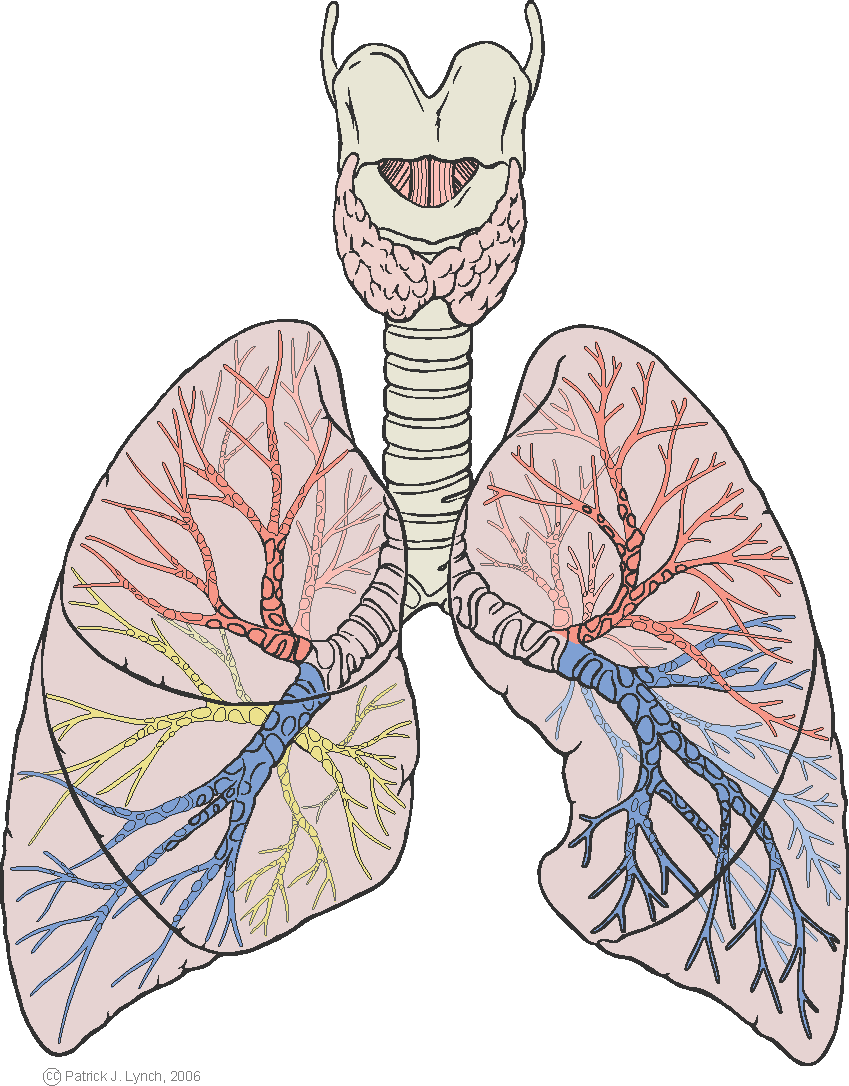
\includegraphics[width=\imsize]{img/Lungs_diagram_detailed}%
		\label{subfig:lung diagram}%
		}%
		\hfill%
	\subfloat[]{%
		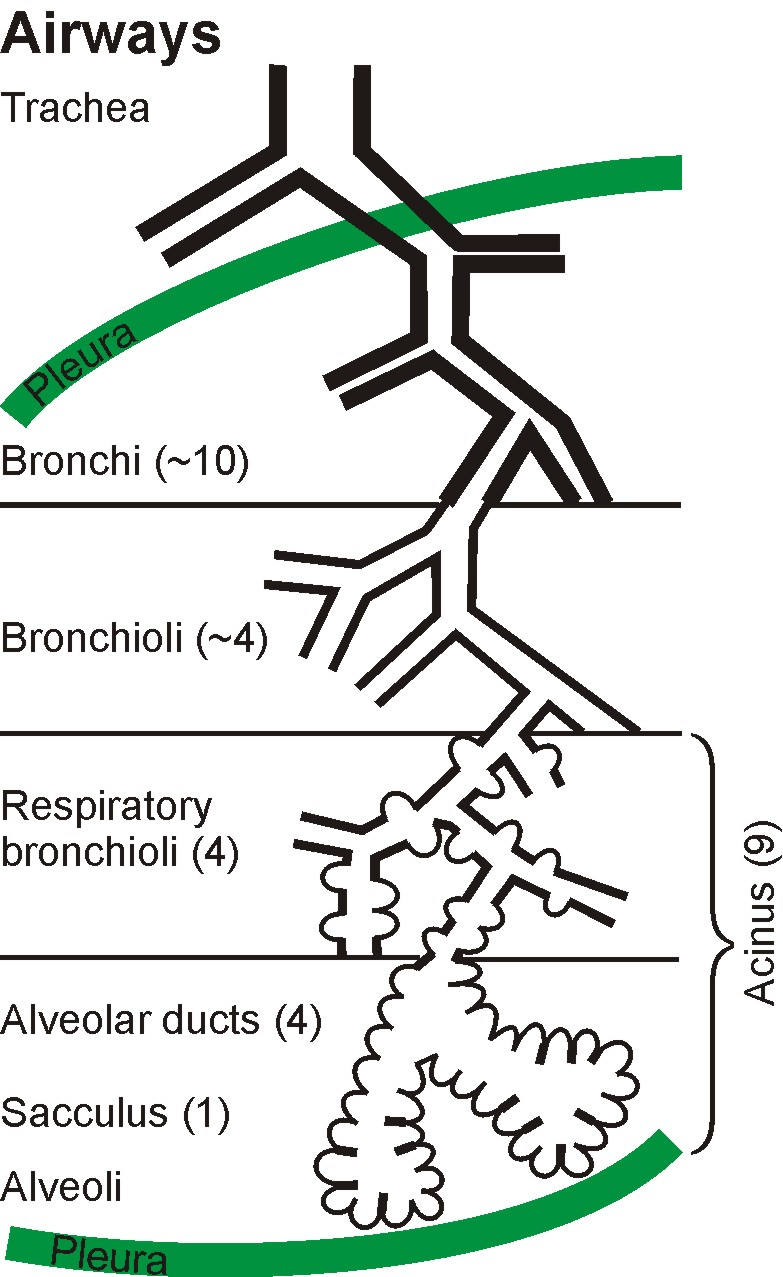
\includegraphics[height=0.6392\linewidth]{img/Lungunits}%
		\label{subfig:lung units}%
		}%
	\caption{Details of the human lung. \subref{subfig:lung diagram}: Lung diagram of the human lung~\cite{LungDiagram}. \subref{subfig:lung units}: Airway generations in the human lung \cite{Schittny2007a}}%
	\label{fig:lung}%
	\todo[inline]{Figure \subref{subfig:lung units} is describing the human lung. Can we put something more ``general'' into it?}
\end{figure}

\section{Why Tomography?}
In our group there has been an ongoing effort to analyze the parenchymal structure of the rat and mouse lung. \citet{Mund2008} challenged the model of aleolarization---the enlargement of the gas exchange surface through lifting off of new septa of the pre-existing septa~\cite{Burri1974}---and developed a working theory on late alveolarization. 

A thorough structural analysis of the lung parenchyma is only possible with three-dimensional data. Traditionally, through stereological methods quantitative information about a three-dimensional structure can be obtaine from measurements performed on two-dimensional planar sections of a sample. Stereology exploits the fact that certain quantities like volume of a certain structure can be determined from the two-dimensional area of said structure in a planar section, \eg\ microscopy slides.

Certain parameters of the lung structure like the topological characteristics of the airway tree, the exact of single acini and which alveolus is ventilated by which alveolar duct cannot be determined using stereological methods\todo{true?}, but need analysis of the three-dimensional relations using tomographic data.